\subsection{TextRank}

TextRank is a graph based unsupervised ranking algorithm formulated for text processing via extracting keywords and sentence extraction from documents. This method is based on Graph-based ranking algorithms like HITS algorithm ~\citep{page1999pagerank} , Google Search Engine's PageRank ~\citep{page1999pagerank} where is used for social networks,  citation analysis and analysis of link structure world wide web. These graph based algorithms exploit the global information computed iteratively rather than looking at only surrounding information. 

The basic idea of the graph based ranking models is `voting' or `recommendation'. If one vertice connected to another vertex, basically it is casting a vote for that other vertex. The higher number of votes the one vertex gets, the same amount of importance it gets. The importance of the vertex which is casting vote is going to determine the amount of importance should be given to that vote. Effectively the score associated with the vertex is determined by votes that are cast for it and scores of vertices that are casting vote for it.

Formally, considering G = (V, E) as directed graph with set of vertices V and set of edges E, where E is the subset of VxV. Let In($V_i$) be the set of vertices that are voting $V_i$ (predecessors) and Out($V_i$) be the set of vertices that $V_i$ is voting to. The score of vertex $V_i$ is calculated  as follows ~\citep{page1999pagerank},

\begin{equation}
S(V_i) = (1-d) + d \sum_{j \in In{V_i}}{\frac{1}{|Out(V_j)|}} * S(V_j)
\end{equation}

here d is called as damping factor that can be set between 0 and 1 initially, which has the role of adding a probability directly jumping from one vertex to another vertex (actually it signifies the default or implicit voting given by any vertex to all other vertices to avoid dead-end in random walk).

Starting from arbitrarily assigned values to all vertices in the graph, the vertex values are computed iterated until convergence or given threshold is reached. After convergence is reached, the scores of the vertices represents the  importance of the vertices within the graph. 

\noindent \textbf{Document as graph}

To use the graph ranking algorithm for natural language text, first we should build a graph that represent the given text and interconnected words and relations between them. Based on the application, text units of various sizes can be used as vertices (examples words, sentences, phrases etc). We can decide type of relations should exist between vertices e.g. lexical or semantic relations, contextual overlap \textit{etc} based application.

Overall steps of this algorithms is, 
\begin{enumerate}

\item Identify the text units of document and add them vertices to the graph.

\item Figure out the relations between text units, that best suits the application. Edges that connects the vertices can be undirected or directed, Weighted or Unweighted.

\item Assign the initial scores of vertices arbitrarily and iterate through ranking algorithm until convergence.

\item Sort the vertices based on final score. and selects top-K vertices as candidate vertices or text units.

\item \lbrack Optional \rbrack Post processing is applied to vertices or textual units.

\end{enumerate}

The expected result of keyword extraction task is set of keywords or phrases for a given natural language text. Any relation between two lexical units can be used as connection between two vertices. Here in this paper, co-occurrence relation with the controlled distance is used as edges or connection between vertices. Two vertices are said to be connected if that two lexical units tend to co-occur within a window of N words, where `N' can vary. 

The vertices added to graph contains lexical units of certain types, for instance in this paper ~\citep{mihalcea2004textrank} they have used individual words as the vertices and connection between vertices (individual words) represents that they co-occurred in the text within the window size N.\\  

\noindent \textbf{Undirected Edges}

Graph used for ranking keyword is undirected, whereas original algorithm was developed for directed graphs. If the two words tend to co-occur then they are mutually connected to each other, so each vetices in-degree equal to out-degree.\\

\noindent \textbf{Weighted Edges}

Edges in the TextRank model is weighted, they directly indicate the strength of connection between two vertices. In this if we two words tend to co-occur frequently then they will have strong (more weight) connection.

By considering above undirected and Weighted cases, the original graph based ranking algorithm has been modified into as follows, 

\begin{equation}
WS(V_i) = (1-d) + d * \sum_{j \in In{V_i}}{\frac{W_{ji}}{\sum_{k \in Out{V_j}{W_{jk}} }}} * WS(V_j)
\end{equation}


\cbox{Example-Text\\}{Apple's product road map is a topic that may receive more speculation than any subject in all of tech. With that in mind, some are expecting 2014 to be a very big year for the Cupertino, Calif.-based maker of the iPad and iPhone.

Jefferies analyst Peter Misek, he of the precarious Apple upgrade, says 2014 will indeed be a crucial year for Apple as the company lays out its next version of the iPhone, the iPhone 6.

Misek notes that the next phone will likely have a new design and a much bigger screen than its predecessor. A 4.8-inch screen is likely size. The iPhone 5s/5c has a 4-inch screen. `We discovered from Asian players that Apple is aggressively investing in OLED alongside its display partners,' Misek wrote in his note. `Apparently Apple has begun to procure equipment for LG Display, Sharp, and Japan Display.'}


\begin{figure}[h]
\begin{center}
\fbox{\scalebox{0.5}{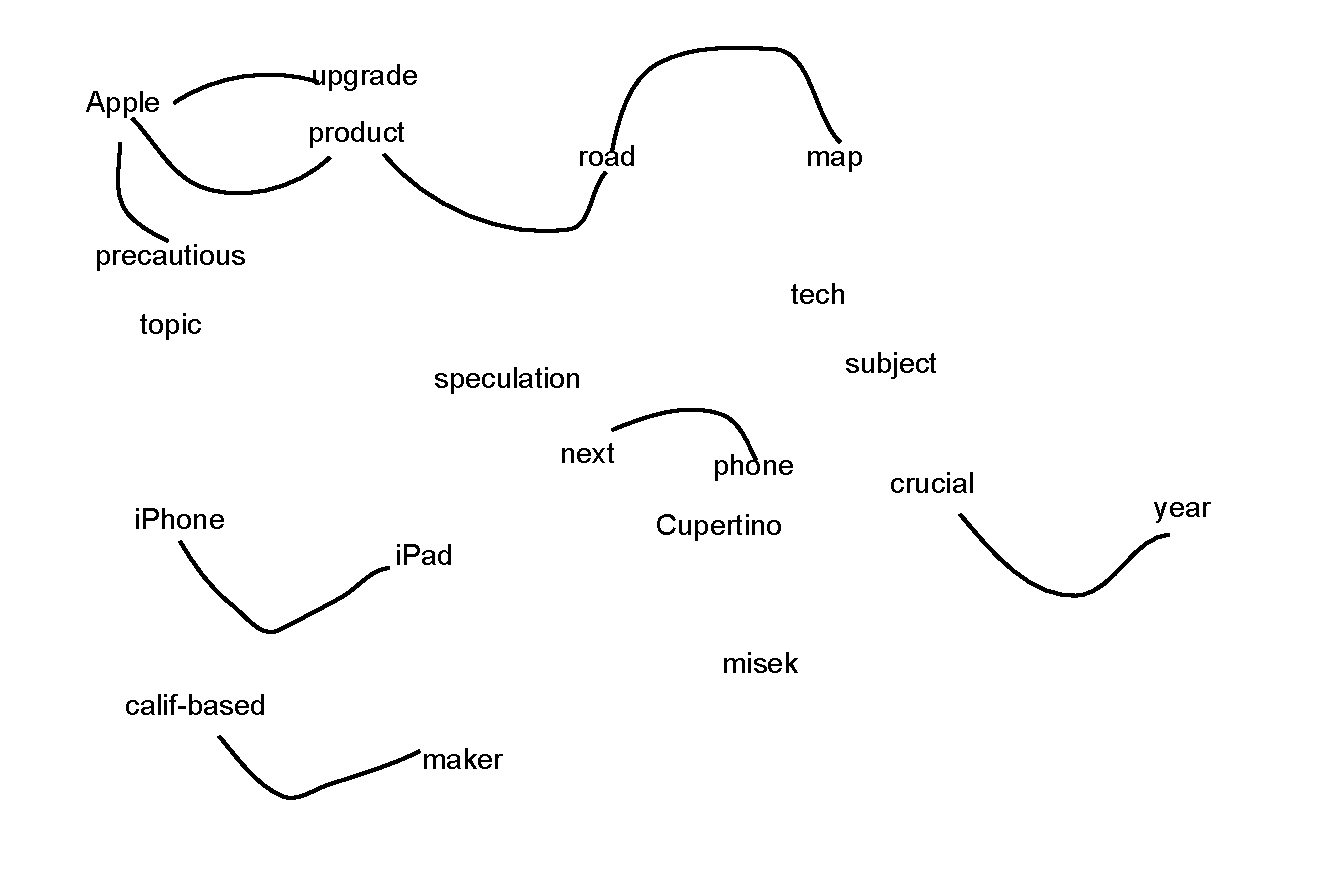
\includegraphics{textrank.pdf}}}
\end{center}
\caption{TextRank - Graph for the above text document}
\end{figure}

\noindent \textbf{Process} 

First the given document is tokenized into words, and syntatic classes of each word (part of speech tag) is identified. It is said that picking only certain syntatic classes gives the better precision (nouns and adjectives). Only unigram words considered as vertices. Graph ranking algorithm run on the constructed  graph. Top fraction of vertices selected based on score given to vertices on convergence. If the selected unigram words tend to co-occur in the text, they are combined together and considered as multi-word keywords or keyphrases.
  
\noindent \textbf{Results} 

This algorithm was tested against 500 science articles where keywords algorithm was compared with manually annotated keywords. It is shown that this algorithm achieves highest F-score 36.2\% when edges are considered as undirected with co-occurence window size (N) is  2.
